\documentclass[12pt,
    a4paper,
    headinclude,
    footinclude]{scrartcl}

    %plainfootsepline

\usepackage{blindtext}
\usepackage[utf8]{inputenc}
\usepackage{setspace}
\usepackage[ngerman]{babel}
\usepackage[ngerman, num]{isodate}
\usepackage[left=3cm,right=2cm,top=2.8cm,bottom=1.6cm]{geometry}

\usepackage{amsmath}  		  % für erw. Formeloptionen, Option [] zur Vermeidung von Type3-Fonts
\usepackage{amstext}          % für Klartext via \text{} in Formeln
\usepackage{amsfonts}         % für komplexere Formeln (Mengensymbole ...)
\usepackage{amssymb}          % für komplexere Formeln (Mengensymbole ...)

\usepackage[style=numeric]{biblatex}
\usepackage[babel,german=guillemets]{csquotes}
\usepackage{graphicx}
\usepackage{listings}
\usepackage{color}
\usepackage{wrapfig}



%kopf und fusszeile
\usepackage[headsepline]{scrpage2}
%\pagestyle{scrheadings} 
\setlength{\footskip}{8mm}
\clearscrheadings
%\ihead{\leftmark}
%\ohead{\rightmark}
%\automark{section}
\cfoot{\pagemark}
%kopf und fusszeile

%Schriftart sfffamily serifenlos
\setkomafont{pageheadfoot}{\normalfont\rmfamily\bfseries}

\setkomafont{section}{\Large\normalfont\rmfamily\bfseries}
\setkomafont{subsection}{\large\normalfont\rmfamily\bfseries}
\setkomafont{subsubsection}{{\normalsize}\normalfont\rmfamily\bfseries}
%Schriftart

\author{Daniel Gilgen, Jan Zschoche}
\title{Numerik}

\begin{document}
	\onehalfspacing
	\monthyearsepgerman{\,}{\,}
	\setcounter{tocdepth}{2}
	
	\begin{titlepage}
	
		\begin{center}
			~\\[0.0cm]
			Berufsakademie Sachsen \\
			Staatliche Studienakadamie Leipzig \\[5cm]
			
			\begin{huge}
				\textbf{Evolutionäre Algorithmen} \\[2cm]
			\end{huge}
			
			\doublespacing
			
			Implementierung eines evolutionären Algorithmus \\
			zur Optimierung der Griewank-Funktion und Untersuchung des Einflusses\\
			 verschiedener Strategien auf die Güte des Ergebnisses\\[3.0cm]
		\end{center}
		
		\onehalfspacing
		\begin{tabbing}
			Eingereicht von: \= ~ \= ~ \= ~ \= Daniel Gilgen \= ~ 5000616\\
			\> \> \> \> Jan Zschoche \> ~ 5000566\\
		\end{tabbing}
		\vspace*{\fill}
		Leipzig, \today
		
	\end{titlepage}
    
    \pagenumbering{arabic}
    \setcounter{page}{1}
    
% Platzproblem !!!!
%	\section{Aufgabe}
%	Es soll ein evolutionärer Algorithmus zur Minimierung der Griewank-Funktion für verschiedene Dimensionen implementiert werden. Diese Funktion besitzt viele lokale Minima und eignet sich daher gut zur Untersuchung von Optimierungsalgorithmen. Das globale Minimum befindet sich, unabhängig von der gewählten Dimension, stets bei $f(\vec{0}) = 0$. Dadurch ist Vergleichbarkeit und die Beurteilung der Ergebnisse gewährleistet. Zusätzlich sollen verschiedene Strategien bezüglich der Elternauswahl, Mutation und Umweltselektion betrachtet werden.
% Platzproblem !!!!
	
	\section{Strategien und Parameter}

	\textbf{Elternauswahl:} Kombination aus rangbasierter und zufälliger Auswahl. Bei der rangbasierten werden die besten 25\% der Population als Grundauswahl herangezogen und aus diesen zufällig Paare gebildet.
	Eine der Strategien wird pro Paarung mit einer bestimmten Wahrscheinlichkeit ausgewählt und zur Anwendung gebracht. Es werden alle Verhältnisse $p_\text{rr}$ der beiden Strategien mit einer Schrittweite von 5\% betrachtet -- $p_\text{rr} = 0$ entspricht rein zufälliger Elternsauswahl, $p_\text{rr} = 1$ rein rangbasierte Elternsauswahl.\\\\	
	\textbf{Mutation:} Es werden zwei Mutationsstrategien betrachtet. \\
	\textbf{Konstant:} bei neu erzeugten Individuen wird jedes Gen mit einer Wahrscheinlichkeit von 50\% mutiert, ältere Individuen werden nicht mutiert.
	\textbf{Altersbasiert ansteigend:} Die Mutationswahrscheinlichkeit eines Allels nimmt beginnend bei 50\% mit steigendem Alter zu.\\
	Im Falle einer Mutation wird das Allel um einen zufälligen (gleichverteilten) Wert zwischen -5 und 5 verschoben. \\\\
	\textbf{Rekombination:} Es wird die intermediäre Rekombination angewendet.\\\\
	\textbf{Umweltselektion:} Aus der Gesamtpopulation werden die ersten 50\% der neuen Generation rangbasiert nach dem Roulette-Verfahren und die zweiten 50\% zufällig ausgewählt. Doppelte Auswahl von Individuen wird ausgeschlossen.\\\\
	\textbf{Parameter:} Die Populationsgröße beträgt 16 und bleibt über alle Generationen konstant. In jeder Generation werden 20 neue Kinder erzeugt.
	
	\section{Ablauf der Untersuchung}
	Die Griewank-Funktion wird für die Dimensionen 2, 4, 8, 16 und 32 minimiert. Jede gewählte Kombination aus Strategien und Dimension wird 50 mal wiederholt. Dabei wird das beste Ergebnis, der Durchschnitt und die Standardabweichung ermittelt. Zusätzlich wird für die vollständig rangbasierte Elternauswahl der Verlauf der Fitness über die Anzahl der Generationen aufgezeichnet. Der Algorithmus wird nach maximal 3000 erzeugten Generationen oder falls die Fitness besser als 0.0001 ist abgebrochen. Auch eine zu geringe Vielfalt der Individuen führt zu einem Abbruch.
\newpage
	\section{Ergebnisse}
	
	\newcommand{\size}{0.78}
	\begin{figure}[!h]
		\begin{center}
			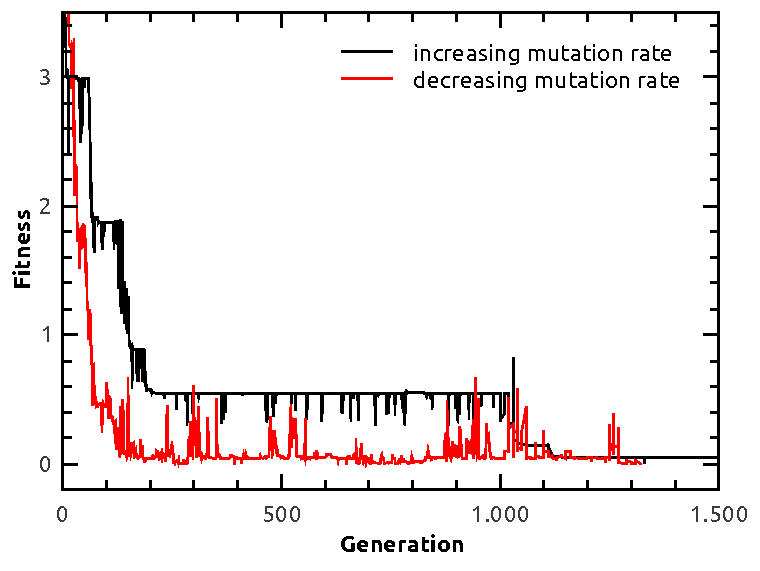
\includegraphics[width=\size\textwidth]{../vortrag/abbildungen/oneCycleAnalysis.pdf}
			\caption{Darstellung der optimalen Fitness in der Population für einen vollständigen evolutionären Zyklus über mehrere Generationen.}
			\label{fig_onecycle}
		\end{center}
	\vspace{-1.cm}
	
	\end{figure}
	\begin{figure}[!h]
		\begin{center}
			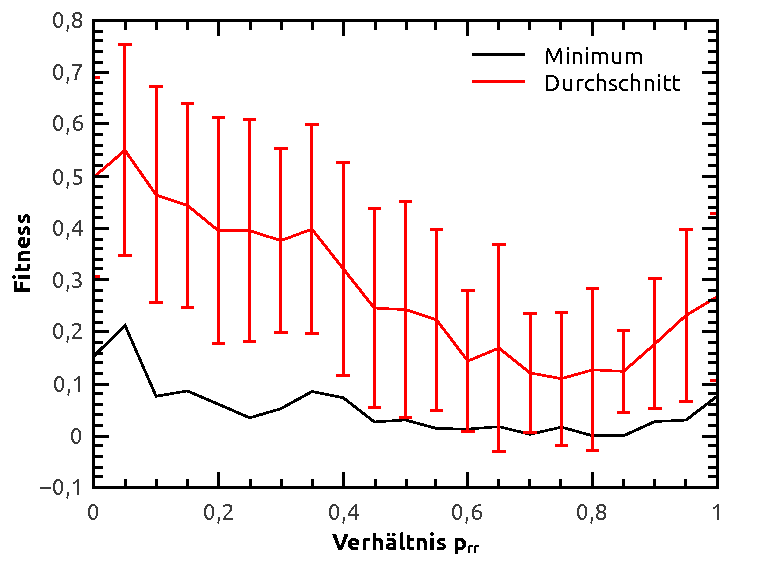
\includegraphics[width=\size\textwidth]{../vortrag/abbildungen/n4_gemittelt_minimal_increasing.pdf}
			\caption{Für jedes Verhältnis $p_\text{rr}$ wurden 10 vollständige Zyklen (vgl. Abb. \ref{fig_onecycle}) berechnet. Beruhend auf diesen 10 Zyklen pro $p_\text{rr}$ werden hier die mittlere Fitness samt Standardabweichung (rot) sowie die beste Fitness (schwarz) dargestellt.}
		\end{center}
	\end{figure}
	\newpage
	
	\begin{figure}[!h]
		\begin{center}
			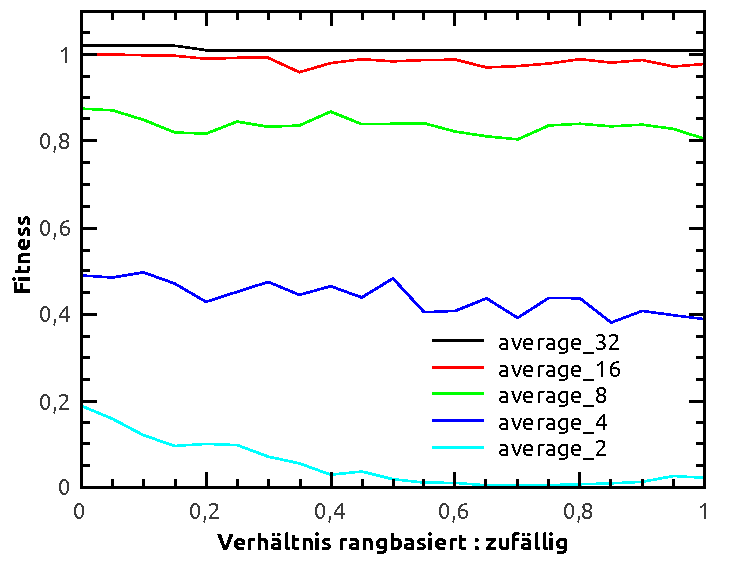
\includegraphics[width=\size\textwidth]{../vortrag/abbildungen/constant_allDim_average.pdf}
			\caption{Darstellung der mittleren Fitness für konstante Mutationsrate und verschiedene Dimensionen der Griewank-Funktion.}
		\end{center}
	\end{figure}

	\begin{figure}[!h]
		\begin{center}
			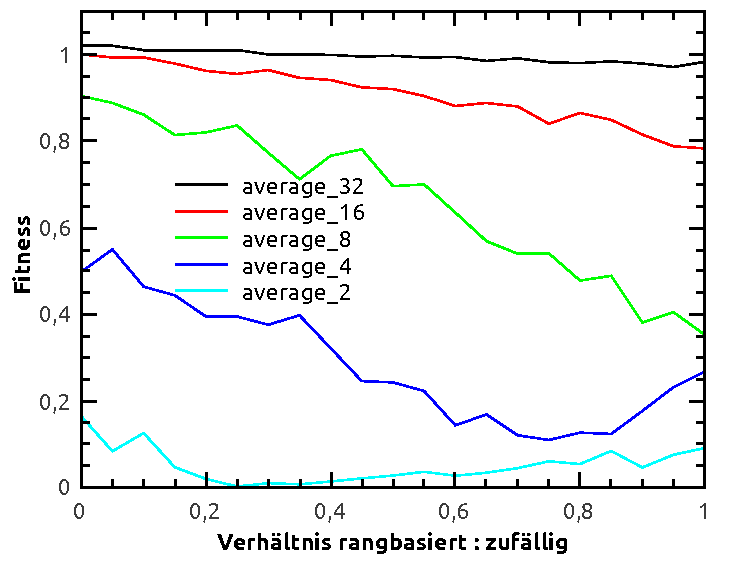
\includegraphics[width=\size\textwidth]{../vortrag/abbildungen/increasing_allDim_average.pdf}
			\caption{Darstellung der mittleren Fitness für konstante Mutationsrate und verschiedene Dimensionen der Griewank-Funktion.}
		\end{center}
	\end{figure}
		
	\begin{figure}[!h]
		\begin{center}
			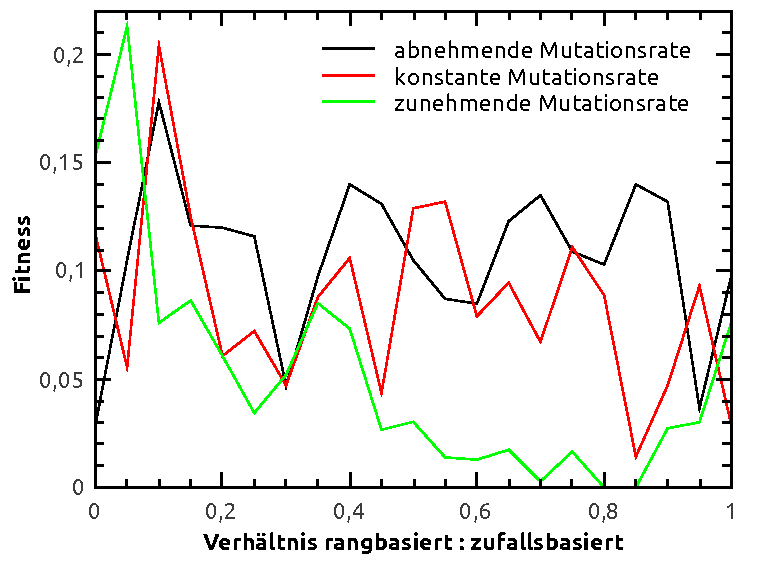
\includegraphics[width=\size\textwidth]{../vortrag/abbildungen/vergleich_mutationsraten_n4.pdf}
			\caption{Vergleich Mutationsstrategien bzgl. der durchschnittlichen Fittness für n=4. }
		\end{center}
	\end{figure}
	\newpage
	\begin{figure}[!h]
		\begin{center}
			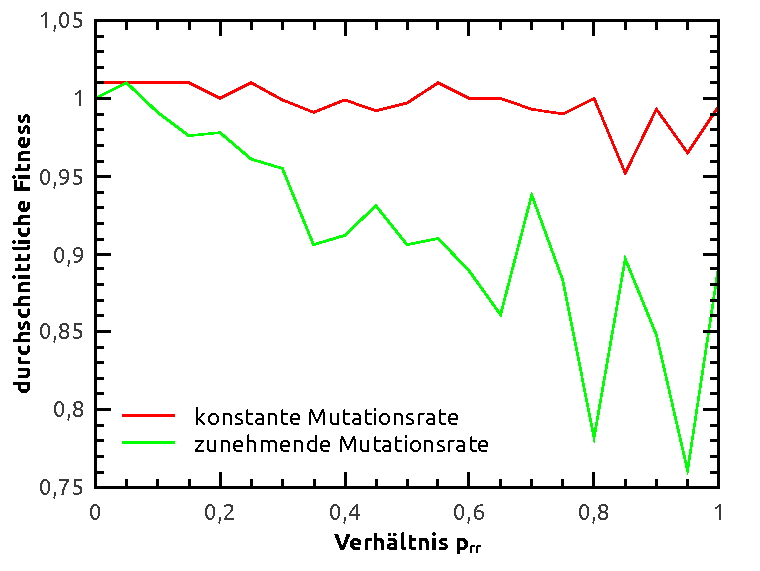
\includegraphics[width=\size\textwidth]{../vortrag/abbildungen/vergleich_mutationsraten_n32.pdf}
			\caption{Vergleich Mutationsstrategien bzgl. der durchschnittlichen Fittness für n=32.}
		\end{center}
	\end{figure}

	\textbf{Zusammenfassung}: Beste Ergebnisse für zunehmende Mutationsrate und einem Rang-Zufallsverhältnis von $p_\text{rr} \approx 0.8$.
	
\end{document}
